\documentclass[a4paperpaper,]{article}
\usepackage{lmodern}
\usepackage{amssymb,amsmath}
\usepackage{ifxetex,ifluatex}
\usepackage{fixltx2e} % provides \textsubscript
\ifnum 0\ifxetex 1\fi\ifluatex 1\fi=0 % if pdftex
  \usepackage[T1]{fontenc}
  \usepackage[utf8]{inputenc}
\else % if luatex or xelatex
  \ifxetex
    \usepackage{mathspec}
  \else
    \usepackage{fontspec}
  \fi
  \defaultfontfeatures{Ligatures=TeX,Scale=MatchLowercase}
\fi
% use upquote if available, for straight quotes in verbatim environments
\IfFileExists{upquote.sty}{\usepackage{upquote}}{}
% use microtype if available
\IfFileExists{microtype.sty}{%
\usepackage{microtype}
\UseMicrotypeSet[protrusion]{basicmath} % disable protrusion for tt fonts
}{}
\usepackage[left=3.75cm, right=3.75cm, top=3cm, bottom=3cm]{geometry}
\usepackage{hyperref}
\PassOptionsToPackage{usenames,dvipsnames}{color} % color is loaded by hyperref
\hypersetup{unicode=true,
            pdftitle={Travaux Pratiques de Biométrie 3},
            pdfauthor={Benoît Simon-Bouhet},
            colorlinks=true,
            linkcolor=Maroon,
            citecolor=Blue,
            urlcolor=blue,
            breaklinks=true}
\urlstyle{same}  % don't use monospace font for urls
\usepackage{natbib}
\bibliographystyle{apalike}
\usepackage{color}
\usepackage{fancyvrb}
\newcommand{\VerbBar}{|}
\newcommand{\VERB}{\Verb[commandchars=\\\{\}]}
\DefineVerbatimEnvironment{Highlighting}{Verbatim}{commandchars=\\\{\}}
% Add ',fontsize=\small' for more characters per line
\usepackage{framed}
\definecolor{shadecolor}{RGB}{247,247,247}
\newenvironment{Shaded}{\begin{snugshade}}{\end{snugshade}}
\newcommand{\AlertTok}[1]{\textcolor[rgb]{0.75,0.01,0.01}{\textbf{\colorbox[rgb]{0.97,0.90,0.90}{#1}}}}
\newcommand{\AnnotationTok}[1]{\textcolor[rgb]{0.79,0.38,0.79}{#1}}
\newcommand{\AttributeTok}[1]{\textcolor[rgb]{0.00,0.34,0.68}{#1}}
\newcommand{\BaseNTok}[1]{\textcolor[rgb]{0.69,0.50,0.00}{#1}}
\newcommand{\BuiltInTok}[1]{\textcolor[rgb]{0.39,0.29,0.61}{\textbf{#1}}}
\newcommand{\CharTok}[1]{\textcolor[rgb]{0.57,0.30,0.62}{#1}}
\newcommand{\CommentTok}[1]{\textcolor[rgb]{0.54,0.53,0.53}{#1}}
\newcommand{\CommentVarTok}[1]{\textcolor[rgb]{0.00,0.58,1.00}{#1}}
\newcommand{\ConstantTok}[1]{\textcolor[rgb]{0.67,0.33,0.00}{#1}}
\newcommand{\ControlFlowTok}[1]{\textcolor[rgb]{0.12,0.11,0.11}{\textbf{#1}}}
\newcommand{\DataTypeTok}[1]{\textcolor[rgb]{0.00,0.34,0.68}{#1}}
\newcommand{\DecValTok}[1]{\textcolor[rgb]{0.69,0.50,0.00}{#1}}
\newcommand{\DocumentationTok}[1]{\textcolor[rgb]{0.38,0.47,0.50}{#1}}
\newcommand{\ErrorTok}[1]{\textcolor[rgb]{0.75,0.01,0.01}{\underline{#1}}}
\newcommand{\ExtensionTok}[1]{\textcolor[rgb]{0.00,0.58,1.00}{\textbf{#1}}}
\newcommand{\FloatTok}[1]{\textcolor[rgb]{0.69,0.50,0.00}{#1}}
\newcommand{\FunctionTok}[1]{\textcolor[rgb]{0.39,0.29,0.61}{#1}}
\newcommand{\ImportTok}[1]{\textcolor[rgb]{1.00,0.33,0.00}{#1}}
\newcommand{\InformationTok}[1]{\textcolor[rgb]{0.69,0.50,0.00}{#1}}
\newcommand{\KeywordTok}[1]{\textcolor[rgb]{0.12,0.11,0.11}{\textbf{#1}}}
\newcommand{\NormalTok}[1]{\textcolor[rgb]{0.12,0.11,0.11}{#1}}
\newcommand{\OperatorTok}[1]{\textcolor[rgb]{0.12,0.11,0.11}{#1}}
\newcommand{\OtherTok}[1]{\textcolor[rgb]{0.00,0.43,0.16}{#1}}
\newcommand{\PreprocessorTok}[1]{\textcolor[rgb]{0.00,0.43,0.16}{#1}}
\newcommand{\RegionMarkerTok}[1]{\textcolor[rgb]{0.00,0.34,0.68}{\colorbox[rgb]{0.88,0.91,0.97}{#1}}}
\newcommand{\SpecialCharTok}[1]{\textcolor[rgb]{0.24,0.68,0.91}{#1}}
\newcommand{\SpecialStringTok}[1]{\textcolor[rgb]{1.00,0.33,0.00}{#1}}
\newcommand{\StringTok}[1]{\textcolor[rgb]{0.75,0.01,0.01}{#1}}
\newcommand{\VariableTok}[1]{\textcolor[rgb]{0.00,0.34,0.68}{#1}}
\newcommand{\VerbatimStringTok}[1]{\textcolor[rgb]{0.75,0.01,0.01}{#1}}
\newcommand{\WarningTok}[1]{\textcolor[rgb]{0.75,0.01,0.01}{#1}}
\usepackage{longtable,booktabs}
\usepackage{graphicx,grffile}
\makeatletter
\def\maxwidth{\ifdim\Gin@nat@width>\linewidth\linewidth\else\Gin@nat@width\fi}
\def\maxheight{\ifdim\Gin@nat@height>\textheight\textheight\else\Gin@nat@height\fi}
\makeatother
% Scale images if necessary, so that they will not overflow the page
% margins by default, and it is still possible to overwrite the defaults
% using explicit options in \includegraphics[width, height, ...]{}
\setkeys{Gin}{width=\maxwidth,height=\maxheight,keepaspectratio}
\IfFileExists{parskip.sty}{%
\usepackage{parskip}
}{% else
\setlength{\parindent}{0pt}
\setlength{\parskip}{6pt plus 2pt minus 1pt}
}
\setlength{\emergencystretch}{3em}  % prevent overfull lines
\providecommand{\tightlist}{%
  \setlength{\itemsep}{0pt}\setlength{\parskip}{0pt}}
\setcounter{secnumdepth}{5}
% Redefines (sub)paragraphs to behave more like sections
\ifx\paragraph\undefined\else
\let\oldparagraph\paragraph
\renewcommand{\paragraph}[1]{\oldparagraph{#1}\mbox{}}
\fi
\ifx\subparagraph\undefined\else
\let\oldsubparagraph\subparagraph
\renewcommand{\subparagraph}[1]{\oldsubparagraph{#1}\mbox{}}
\fi

%%% Use protect on footnotes to avoid problems with footnotes in titles
\let\rmarkdownfootnote\footnote%
\def\footnote{\protect\rmarkdownfootnote}

%%% Change title format to be more compact
\usepackage{titling}

% Create subtitle command for use in maketitle
\newcommand{\subtitle}[1]{
  \posttitle{
    \begin{center}\large#1\end{center}
    }
}

\setlength{\droptitle}{-2em}

  \title{Travaux Pratiques de Biométrie 3}
    \pretitle{\vspace{\droptitle}\centering\huge}
  \posttitle{\par}
    \author{Benoît Simon-Bouhet}
    \preauthor{\centering\large\emph}
  \postauthor{\par}
      \predate{\centering\large\emph}
  \postdate{\par}
    \date{2019-03-03}

\usepackage[french]{babel}
\usepackage{mathspec}  % \usepackage{fontspec}
\usepackage{natbib}

\usepackage{setspace,booktabs,rotating,placeins,hvfloat,textcomp}

\usepackage{graphicx}
\usepackage{multicol}
\usepackage{enumitem}
\usepackage{longtable}

\setallmainfonts[Ligatures = TeX]{FuturaLT-Book}
\onehalfspace

\begin{document}
\maketitle

{
\hypersetup{linkcolor=black}
\setcounter{tocdepth}{2}
\tableofcontents
}
\hypertarget{preambule}{%
\section{Préambule}\label{preambule}}

Ce livre contient l'ensemble du matériel (contenus, exemples, exercices\ldots{}) nécessaire à la réalisation des travaux pratiques et TEA de biométrie 3. Ces travaux pratiques ont un seul objectif principal : vous permettre de mettre en œuvre, dans \texttt{RStudio} les méthodes statistiques découvertes en cours magistral et en TD de biométrie 2 (au semestre précédent) et en biométrie 3 depuis début janvier.

Je considère qu'à ce stade, vous devez être à l'aise dans RStudio pour effectuer les tâches suivantes :

\begin{enumerate}
\def\labelenumi{\arabic{enumi}.}
\tightlist
\item
  Importer des jeux de données dans RStudio
\item
  Manipuler des tableaux de données avec \texttt{tidyr} pour les mettre dans un format permettant les analyses statistiques et les représentations graphiques
\item
  Faire des graphiques exploratoires avec \texttt{ggplot2} pour visualiser des données
\item
  Filtrer des lignes, sélectionner des colonnes, trier, créer de nouvelles variables et calculer des résumés des données avec les fonction \texttt{filter()}, \texttt{select()}, \texttt{arrange()}, \texttt{mutate()}, \texttt{summarise()} et \texttt{group\_by()} du package \texttt{dplyr}
\item
  Utiliser le pipe \texttt{\%\textgreater{}\%} afin d'enchaîner plusieurs commandes
\item
  Créer des scripts parlants contenant des commandes et des commentaires utiles
\item
  Spécifier/modifier votre répertoire de travail
\item
  Installer des packages additionnels.
\end{enumerate}

Si vous pensez avoir besoin de rappels sur ces notions, je vous encourrage vivement à consulter \href{https://besibo.github.io/Biometrie2/}{le livre en ligne} dédié aux travaux pratiques de Biométrie 2 pour vous rafraîchir la mémoire.

L'organisation des TP et TEA de biométrie 3 sera la suivante :

\begin{itemize}
\tightlist
\item
  Séance 1 : 1h30 de TP suivie d'une séance de 1h30 de TEA. Rappels concernant les statistiques descriptives et les visualisations graphiques utiles pour déméler la complexité de certains jeux de données. Comparaisons (paramétriques et non paramétriques) de la moyenne de 2 populations.
\item
  Séance 2 : 1h30 de TP suivie d'une séance de 1h30 de TEA. Comparaisons (paramétriques et non paramétriques) la moyenne de plus de 2 populations : analyse de variance, hypothèses et conditions d'application.
\item
  Séance 3 : 1h30 de TP suivie d'une séance de 1h30 de TEA. Étude de la liaison entre 2 variables. Corrélation (paramétrique et non paramétrique) et régression linéaire. Tests d'hypothèses, estimation et conditions d'application.
\item
  Séance 4 : 1h30 de TP. Exercices d'application et corrections en guise de préparation pour l'examen.
\end{itemize}

\hypertarget{intro}{%
\section{Introduction}\label{intro}}

Sur votre disque dur, créez un dossier nommé ``Biometrie3'' (sans accent, sans espace).
Au début de chaque nouvelle séance de TP, vous devrez ensuite effectuer les opérations suivantes :

\begin{enumerate}
\def\labelenumi{\arabic{enumi}.}
\tightlist
\item
  Créez, dans votre dossier ``Biometrie3'', un sous-dossier nommé ``TP\_1'', ``TP\_2'', etc.
\item
  Téléchargez les fichiers utiles disponibles sur l'ENT et placez-les dans le dossier du TP correspondant.
\item
  Lancez RStudio.
\item
  Dans l'onglet ``Files'' de RStudio, naviguez jusqu'au sous-dossier ``TP\_X'' que vous venez de créer et indiquez à RStudio qu'il s'agit de votre répertoire de travail. Si vous ne savez plus comment faire, consultez \href{https://besibo.github.io/Biometrie2/bases.html\#le-repertoire-de-travail}{la section 2.2.2} du livre en ligne de Biométrie 2. Si votre répertoire de travail a été correctement spécifié, vous devriez constater qu'une commande ressemblant à ceci est apparue dans la console de RStudio :
\end{enumerate}

\begin{Shaded}
\begin{Highlighting}[]
\KeywordTok{setwd}\NormalTok{(}\StringTok{"C:/.........../Biometrie3/TP_X"}\NormalTok{)}
\end{Highlighting}
\end{Shaded}

\begin{enumerate}
\def\labelenumi{\arabic{enumi}.}
\setcounter{enumi}{4}
\tightlist
\item
  Dans la console, tapez :
\end{enumerate}

\begin{Shaded}
\begin{Highlighting}[]
\KeywordTok{list.files}\NormalTok{()}
\end{Highlighting}
\end{Shaded}

La liste des fichiers contenus dans votre répertoire de travail (donc le nom des fichiers que vous avez téléchargé sur l'ENT) devrait apparaître dans la console. Si ce n'est pas le cas, recommencez depuis le début. Vous pouvez également vérifier à tout moment si le répertoire de travail utilisé par RStudio est bien celui que vous pensez en tapant :

\begin{Shaded}
\begin{Highlighting}[]
\KeywordTok{getwd}\NormalTok{()}
\end{Highlighting}
\end{Shaded}

\begin{enumerate}
\def\labelenumi{\arabic{enumi}.}
\setcounter{enumi}{5}
\tightlist
\item
  Créez un nouveau script dans votre répertoire de travail et sauvegardez-le. Si vous ne savez plus comment faire, consultez \href{https://besibo.github.io/Biometrie2/bases.html\#les-scripts}{la section 2.2.3} du livre en ligne de Biométrie 2.
\item
  Dans l'onglet ``History'' de RStudio, cliquez sur la commande commençant par \texttt{setwd()} puis cliquez sur le bouton ``To source'' (une flèche verte dirigée vers la gauche). Cela a pour effet de copier dans votre script la commande permettant de spécifier le répertoire de travail correct. Ainsi, lors de votre prochaine session de travail, vous n'aurez pas besoin de spécifier manuellement quel est votre répertoire de travail comme nous l'avons fait à l'étape 4 ci-dessus : il vous suffira d'ouvrir votre script et d'envoyer cette commande dans la console en pressant les touches \texttt{ctrl\ +\ Entrée}.
\item
  N'oubliez pas de sauvegarder votre script très régulièrement et d'y ajouter autant de commentaires que nécessaire avec le symbole \texttt{\#}.
\end{enumerate}

Si vous suivez rigoureusement ces étapes, vous devriez être dans la situation idéale pour commencer à travailler efficacement dans RStudio. Avec un minimum d'habitude, mettre tout ça en place ne devrait pas vous demander plus de 2 ou 3 minutes. À partir de maintenant, toutes vos analyses et commentaires doivent figurer dans vos scripts.

\hypertarget{seance-1-statistiques-descriptives-et-tests-dhypotheses}{%
\section{Séance 1 : statistiques descriptives et tests d'hypothèses}\label{seance-1-statistiques-descriptives-et-tests-dhypotheses}}

\hypertarget{packages-et-donnees}{%
\subsection{Packages et données}\label{packages-et-donnees}}

Pour chacune des 4 séances de travaux pratiques (et TEA) qui viennent, vous aurez besoin d'utiliser des packages spécifiques et d'importer des données depuis des fichiers externes disponibles sur l'ENT.

Les packages dont vous aurez besoin pour cette séance, et que vous devez donc charger en mémoire, sont les suivants :

\begin{Shaded}
\begin{Highlighting}[]
\KeywordTok{library}\NormalTok{(tidyverse)}
\KeywordTok{library}\NormalTok{(readr)}
\KeywordTok{library}\NormalTok{(skimr)}
\end{Highlighting}
\end{Shaded}

Si ces commandes (que vous devez taper dans vos scripts avant de les exécuter dans la console de RStudio) renvoient des messages d'erreur, c'est que les packages que vous essayez de charger en mémoire ne sont pas installés sur votre ordinateur. Il vous faudra alors installer les packages manquants avec la fonction :

\begin{Shaded}
\begin{Highlighting}[]
\KeywordTok{install.packages}\NormalTok{(}\StringTok{"nom_du_package"}\NormalTok{)}
\end{Highlighting}
\end{Shaded}

Comme d'habitude, si tout ça est un peu flou pour vous, relisez \href{https://besibo.github.io/Biometrie2/bases.html\#charger-un-package-en-memoire}{la section 2.3} du livre de biométrie 2 disponible en ligne.

Vous aurez également besoin des jeux de données suivants :

\begin{itemize}
\tightlist
\item
  \texttt{Temperature.csv}
\item
  \texttt{Testosterone.csv}
\item
  \texttt{HornedLizards.csv}
\item
  \texttt{HommesFemmes.txt}
\end{itemize}

\hypertarget{comparaison-de-la-moyenne-dune-population-a-une-valeur-theorique}{%
\subsection{Comparaison de la moyenne d'une population à une valeur théorique}\label{comparaison-de-la-moyenne-dune-population-a-une-valeur-theorique}}

\hypertarget{Explo}{%
\subsubsection{Exploration préalable des données}\label{Explo}}

Avant de se lancer dans les tests d'hypothèses, il est \textbf{toujours indispensable} d'examiner les données dont on dispose à l'aide, d'une part de statistiques descriptives numériques, et d'autres part, de graphiques exploratoires. Nous allons voir dans cette section quels indices statistiques il peut être utile de calculer et quelles représentations graphiques il peut être utile de réaliser afin de pouvoir se lancer dans des tests d'hypothèses risquer de grossières erreurs.

\hypertarget{importation-et-examen-visuel}{%
\paragraph{Importation et examen visuel}\label{importation-et-examen-visuel}}

Commencez par importer les données contenues dans le fichier \texttt{Temperature.csv}. Pour cela, utilisez l'assistant d'importation de RStudio. Si vous ne savez plus comment faire, consultez \href{https://besibo.github.io/Biometrie2/tidyr.html\#importer-des-donnees-depuis-un-tableur}{la section 5.3} du livre en ligne de Biométrie 2.

Vous stockerez les données dans un objet que vous nommerez \texttt{Temperature}. Après l'importation, taper son nom dans la console de RStudio doit produire le résultat suivant :

\begin{Shaded}
\begin{Highlighting}[]
\NormalTok{Temperature}
\end{Highlighting}
\end{Shaded}

\begin{verbatim}
# A tibble: 25 x 2
   individual temperature
        <dbl>       <dbl>
 1          1        98.4
 2          2        98.6
 3          3        97.8
 4          4        98.8
 5          5        97.9
 6          6        99  
 7          7        98.2
 8          8        98.8
 9          9        98.8
10         10        99  
# ... with 15 more rows
\end{verbatim}

Ce tableau contient les températures corporelles de 25 adultes en bonne santé choisis au hasard parmi la population américaine. On souhaite examiner la croyance populaire indiquant que la température moyenne d'adultes en bomme santé vaut 37ºC.

La première chose à faire quand on travaille avec des données inconnues, c'est d'examiner les données brutes. Ici, les données sont importées au format \texttt{tibble}, donc seules les premières lignes sont visibles. Pour visualiser l'ensemble du tableau, utilisez la fonction \texttt{View()} :

\begin{Shaded}
\begin{Highlighting}[]
\KeywordTok{View}\NormalTok{(Temperature)}
\end{Highlighting}
\end{Shaded}

Cette commande doit ouvrir un nouvel onglet présentant les données dans un tableur simplifié, en lecture seule.

On constate ici 2 choses que nous allons modifier :

\begin{enumerate}
\def\labelenumi{\arabic{enumi}.}
\tightlist
\item
  la première colonne, intitulé \texttt{inidividual}, n'est pas véritablement une variable. Cette colonne ne contient qu'un identifiant qui est en fait identique au numéro de ligne. Nous allons donc supprimer cette colonne
\item
  les températures sont exprimées en degrés Fahrenheit, ce qui rend leur lecture difficile pour nous qui sommes habitués à utiliser le système métrique et les degrés Celsius. Nous allons donc convertir les températures en degrés Celsius grâce à la formule suivante :
\end{enumerate}

\[ºC = \frac{ºF - 32}{1.8}\]

\begin{Shaded}
\begin{Highlighting}[]
\NormalTok{Temp_clean <-}\StringTok{ }\NormalTok{Temperature }\OperatorTok\StringTok{ }
\StringTok{  }\KeywordTok{select}\NormalTok{(}\OperatorTok{-}\NormalTok{individual) }\OperatorTok\StringTok{      }\CommentTok{# Suppression de la première colonne}
\StringTok{  }\KeywordTok{mutate}\NormalTok{(                      }\CommentTok{# Transformation des tempértures en Celsius}
    \DataTypeTok{temperature =}\NormalTok{ (temperature }\OperatorTok{-}\StringTok{ }\DecValTok{32}\NormalTok{) }\OperatorTok{/}\StringTok{ }\FloatTok{1.8}
\NormalTok{    )}

\NormalTok{Temp_clean}
\end{Highlighting}
\end{Shaded}

\begin{verbatim}
# A tibble: 25 x 1
   temperature
         <dbl>
 1        36.9
 2        37.0
 3        36.6
 4        37.1
 5        36.6
 6        37.2
 7        36.8
 8        37.1
 9        37.1
10        37.2
# ... with 15 more rows
\end{verbatim}

Il nous est maintenant possible d'examiner à nouveau les données avec la fonction \texttt{View()}. Avec des valeurs de températures comprises entre 36.3 ºC et 37.8 ºC, il n'y a visiblement pas de données aberrantes.

C'est toujours la première chose à faire : regarder les données brutes pour repérer :
- La nature des variables présentes.
- Les variables inutiles qui pourront être supprimées ou négligées.
- Les unités des variables utiles, afin de pouvoir les convertir si nécessaire.
- Les valeurs manquantes ou aberrantes qui demanderont toujours un soin particulier.

Une fois l'examen préliminaire des données réalisé, on peut passer au calcul des statistiques descriptives.

\hypertarget{statistiques-descriptives}{%
\paragraph{Statistiques descriptives}\label{statistiques-descriptives}}

On s'intéresse ici au calcul de grandeurs statistiques nous apportant des renseignement sur la distribution des valeurs de l'échantillon. Les questions auxquelles on tente de répondre à ce stade sont les suivantes :

\begin{itemize}
\tightlist
\item
  Quelle est la tendance moyenne
\item
  Quelle est la dispersion des données autour de la moyenne
\end{itemize}

Pour répondre à ces questions, on peut faire appel à de multiples fonctions. J'en évoquerai ici seulement 3 qui permettent d'obtenir la plupart des informations dont nous avons besoin très simplement :

\begin{Shaded}
\begin{Highlighting}[]
\KeywordTok{summary}\NormalTok{(Temp_clean)}
\end{Highlighting}
\end{Shaded}

\begin{verbatim}
  temperature   
 Min.   :36.33  
 1st Qu.:36.67  
 Median :37.00  
 Mean   :36.96  
 3rd Qu.:37.22  
 Max.   :37.78  
\end{verbatim}

Comme son nom l'indique, la fonction \texttt{summary()} renvoie un résumé des données :

\begin{itemize}
\tightlist
\item
  les valeurs extrêmes (minimum et maximum)
\item
  les valeurs ``centrales'' (moyenne et médiane)
\item
  les valeurs des quartiles (premier et troisième quartiles)
\end{itemize}

Ces valeurs seront presques toutes reprises sur le graphique de type ``boîte à moustaches'' que nous verrons plus bas.

On constate ici que la moyenne et la médiane sont très proches. La distribution des température doit donc être à peut près symmétrique, avec à peu près autant de valeurs au dessus que de valeurs en dessous de la moyenne.

La seconde fonction utile est la fonction \texttt{IQR()}, comme ``Inter Quartile Range'' (ou intervalle inter-quartile). Cette fonction renvoie l'étendue de l'intervalle inter-quartile, c'est à dire la valeur du troisième quartile moins la valeur de premier quartile. Attention, cette fonction a besoin d'un vecteur en guise d'argument, or nos données sont stockées sous forme de \texttt{tibble}. Nous allons donc utiliser la fonction \texttt{pull()} du package \texttt{dplyr} afin de transformer (momentanément) la colonne \texttt{temperature} du tableau \texttt{Temp\_clean} en vecteur :

\begin{Shaded}
\begin{Highlighting}[]
\NormalTok{Temp_clean }\OperatorTok\StringTok{ }\KeywordTok{pull}\NormalTok{(temperature) }\OperatorTok\StringTok{ }\KeywordTok{IQR}\NormalTok{()}
\end{Highlighting}
\end{Shaded}

\begin{verbatim}
[1] 0.5555556
\end{verbatim}

On constate ici que l'intervalle inter quartile a une largeur de 0.55 degrés Celsius. Cela signifie que les 50\% des températures les plus centrales sont situées dans un intervalle d'environ un demi-degré celsius.

Enfin, un eautre façon d'obtenir des informations rapidement consiste à utiliser la fonction \texttt{skim()} du package \texttt{skimr} :

\begin{Shaded}
\begin{Highlighting}[]
\KeywordTok{skim}\NormalTok{(Temp_clean)}
\end{Highlighting}
\end{Shaded}

\begin{verbatim}
Skim summary statistics
 n obs: 25 
 n variables: 1 

-- Variable type:numeric -----------------------------------------------------------
    variable missing complete  n  mean   sd    p0   p25 p50   p75
 temperature       0       25 25 36.96 0.38 36.33 36.67  37 37.22
  p100     hist
 37.78 ▅▃▁▇▇▂▂▁
\end{verbatim}

(Attention : si vous lisez ce document au format pdf, vous ne pourrez pas visualiser correctement la totalité des résultats produits par cette fonction. Consultez la version html de ce document, ou tapez la commande dans RStudio).

Toute comme \texttt{summary()}, la fonction \texttt{skim()} renvoie les valeurs minimales et maximales, les premiers et troisièmes quartiles ainsi que la moyenne et la médiane. Elle nous indique en outre la valeur de l'écart-type de l'échantillon, ainsi que le nombre d'observation et le nombre de données manquantes. Enfin, elle fournit un histogramme très schématique et sans échelle. Cet histogramme nous permet de nous faire une première idée de la distribution des données.

Outre ces 3 fonctions (\texttt{summary()}, \texttt{IQR()}, et \texttt{skim()}), il est bien sûr possible de calculer toutes ces valeurs manuellement si besoin :

\begin{itemize}
\tightlist
\item
  \texttt{mean()} permet de calculer la moyenne
\item
  \texttt{median()} permet de calculer la médiane
\item
  \texttt{min()} et \texttt{max()} permettent de calculer les valeurs minimales et maximales respectivement
\item
  \texttt{quantile()} permet de calculer les quartiles
\item
  \texttt{sd()} permet de calculer l'écart-type
\item
  \texttt{var()} permet de calculer la variance
\end{itemize}

Toutes ces fonctions prennent seulement un vecteur en guise d'argument. Il faut donc procéder comme avec \texttt{IQR()} pour les utiliser. Par exemple, pour calculer la variance, on peut taper :

\begin{Shaded}
\begin{Highlighting}[]
\NormalTok{Temp_clean }\OperatorTok\StringTok{ }\KeywordTok{pull}\NormalTok{(temperature) }\OperatorTok\StringTok{ }\KeywordTok{var}\NormalTok{()}
\end{Highlighting}
\end{Shaded}

\begin{verbatim}
[1] 0.1417901
\end{verbatim}

ou :

\begin{Shaded}
\begin{Highlighting}[]
\KeywordTok{var}\NormalTok{(Temp_clean}\OperatorTok{$}\NormalTok{temperature)}
\end{Highlighting}
\end{Shaded}

\begin{verbatim}
[1] 0.1417901
\end{verbatim}

\hypertarget{exploration-graphique}{%
\paragraph{Exploration graphique}\label{exploration-graphique}}

Ici, il s'agit d'examiner la distribution des données. Pour cela, 3 types de graphiques sont généralement utilisés.

\begin{enumerate}
\def\labelenumi{\arabic{enumi}.}
\tightlist
\item
  Les nuages de points ou stripcharts :
\end{enumerate}

\begin{Shaded}
\begin{Highlighting}[]
\NormalTok{Temp_clean }\OperatorTok\StringTok{ }
\StringTok{  }\KeywordTok{ggplot}\NormalTok{(}\KeywordTok{aes}\NormalTok{(}\DataTypeTok{x =} \DecValTok{1}\NormalTok{, }\DataTypeTok{y =}\NormalTok{ temperature)) }\OperatorTok{+}
\StringTok{  }\KeywordTok{geom_point}\NormalTok{()}
\end{Highlighting}
\end{Shaded}

\begin{center}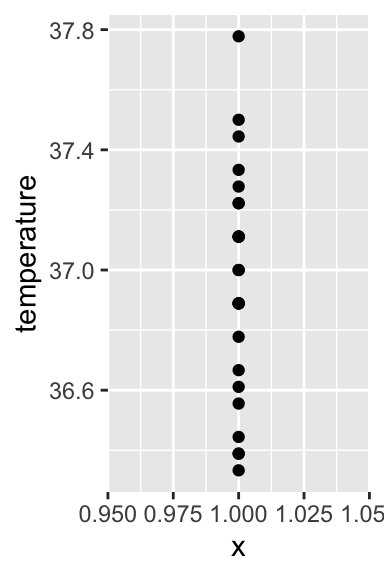
\includegraphics[width=0.25\linewidth]{figure/unnamed-chunk-15-1} \end{center}

Dans la mesure ou souvent, plusieurs observations ont la même valeur, il faut tenir compte de l'over-plotting. Si vous ne vous rappelez plus de quoi il s'agit, consultez \href{https://besibo.github.io/DA/viz.html\#over-plotting}{la section 4.3.4} du livre en ligne de Biométrie 2. Globalement, pour visualiser correctement les données, on va jouer soit sur la transparence des points, soit sur l'ajout d'un bruit aléatoire horizontal qui permettra de distinguer plsu facilement les points,m et de repérer les zones où les points sont abondants ou rares :

\begin{Shaded}
\begin{Highlighting}[]
\NormalTok{Temp_clean }\OperatorTok\StringTok{ }
\StringTok{  }\KeywordTok{ggplot}\NormalTok{(}\KeywordTok{aes}\NormalTok{(}\DataTypeTok{x =} \DecValTok{1}\NormalTok{, }\DataTypeTok{y =}\NormalTok{ temperature)) }\OperatorTok{+}
\StringTok{  }\KeywordTok{geom_jitter}\NormalTok{(}\DataTypeTok{height =} \DecValTok{0}\NormalTok{, }\DataTypeTok{width =} \FloatTok{0.1}\NormalTok{) }\OperatorTok{+}
\StringTok{  }\KeywordTok{xlim}\NormalTok{(}\FloatTok{0.5}\NormalTok{, }\FloatTok{1.5}\NormalTok{)}
\end{Highlighting}
\end{Shaded}

\begin{center}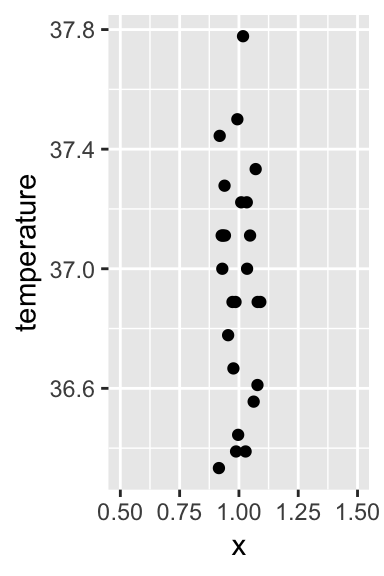
\includegraphics[width=0.25\linewidth]{figure/unnamed-chunk-16-1} \end{center}

La fonction \texttt{xlim()} permet de spéccifier manuellement les valeurs limites que l'on souhaite pour l'axe des abscisses. Ici, cet axe n'a aucune signification particulière puisque nous n'avons qu'une unique série de données (c'est la raison pour laquelle les points sont centrés sur l'abscisse x = 1). Nous pouvons donc le masquer comme ceci :

\begin{Shaded}
\begin{Highlighting}[]
\NormalTok{Temp_clean }\OperatorTok\StringTok{ }
\StringTok{  }\KeywordTok{ggplot}\NormalTok{(}\KeywordTok{aes}\NormalTok{(}\DataTypeTok{x =} \DecValTok{1}\NormalTok{, }\DataTypeTok{y =}\NormalTok{ temperature)) }\OperatorTok{+}
\StringTok{  }\KeywordTok{geom_jitter}\NormalTok{(}\DataTypeTok{height =} \DecValTok{0}\NormalTok{, }\DataTypeTok{width =} \FloatTok{0.1}\NormalTok{) }\OperatorTok{+}
\StringTok{  }\KeywordTok{xlim}\NormalTok{(}\FloatTok{0.5}\NormalTok{, }\FloatTok{1.5}\NormalTok{) }\OperatorTok{+}
\StringTok{  }\KeywordTok{theme}\NormalTok{(}\DataTypeTok{axis.text.x =} \KeywordTok{element_blank}\NormalTok{(),}
        \DataTypeTok{axis.ticks.x =} \KeywordTok{element_blank}\NormalTok{(),}
        \DataTypeTok{axis.title.x =} \KeywordTok{element_blank}\NormalTok{())}
\end{Highlighting}
\end{Shaded}

\begin{center}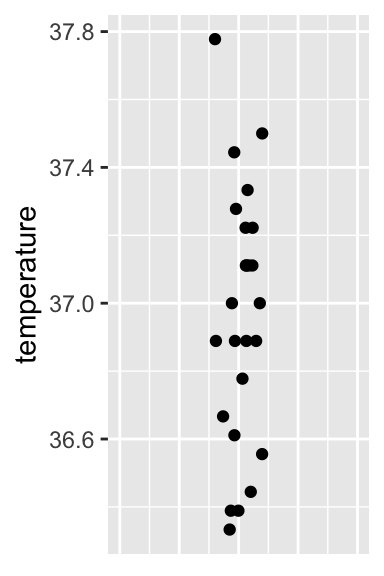
\includegraphics[width=0.25\linewidth]{figure/unnamed-chunk-17-1} \end{center}

On constate ici que la répartition des points est assez régulière, avec néanmoins une majorité de points entre 36.8 et 37.3 degrés Celsius.

\begin{enumerate}
\def\labelenumi{\arabic{enumi}.}
\setcounter{enumi}{1}
\tightlist
\item
  L'histogramme :
\end{enumerate}

\begin{Shaded}
\begin{Highlighting}[]
\NormalTok{Temp_clean }\OperatorTok\StringTok{ }
\StringTok{  }\KeywordTok{ggplot}\NormalTok{(}\KeywordTok{aes}\NormalTok{(}\DataTypeTok{x =}\NormalTok{ temperature)) }\OperatorTok{+}
\StringTok{  }\KeywordTok{geom_histogram}\NormalTok{(}\DataTypeTok{bins =} \DecValTok{10}\NormalTok{, }\DataTypeTok{color =} \KeywordTok{grey}\NormalTok{(}\FloatTok{0.8}\NormalTok{))}
\end{Highlighting}
\end{Shaded}

\begin{center}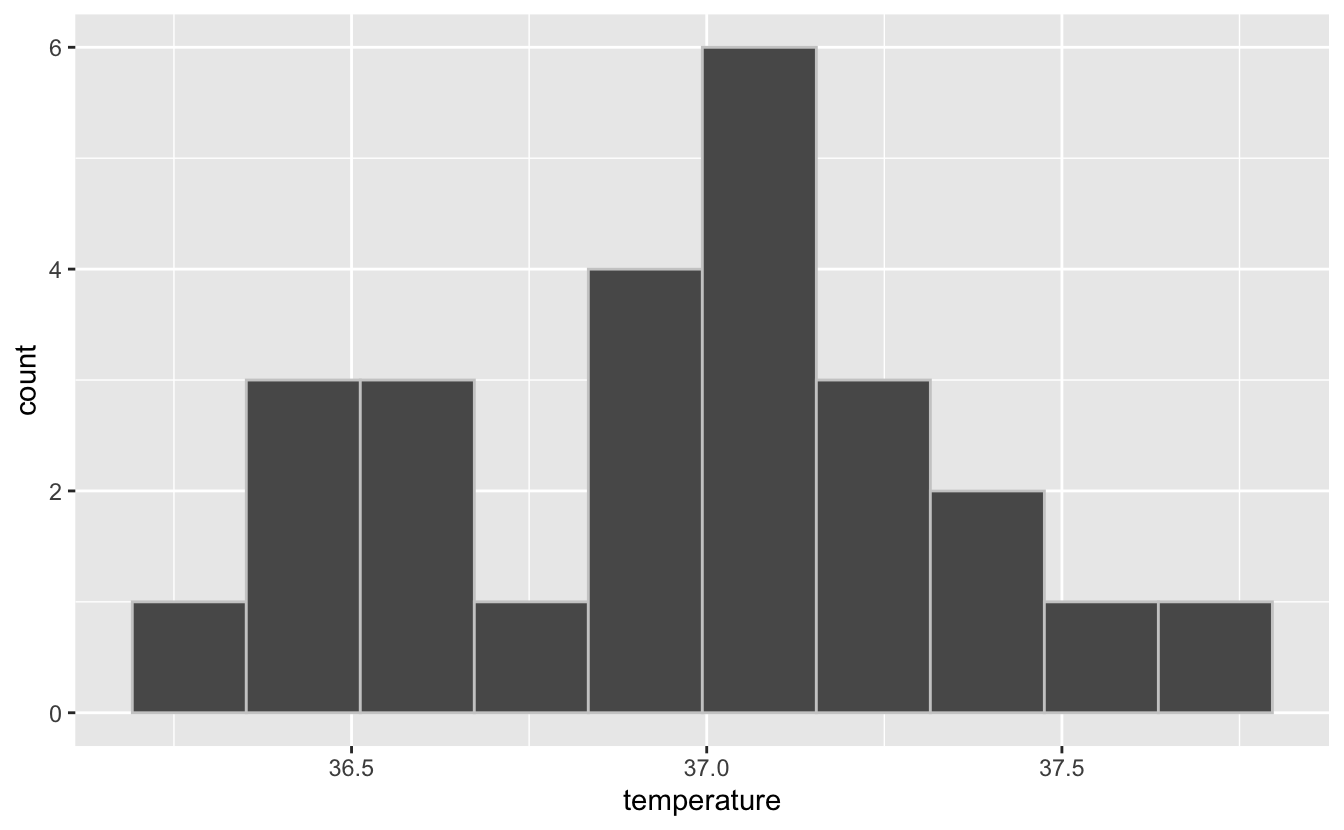
\includegraphics[width=0.9\linewidth]{figure/unnamed-chunk-18-1} \end{center}

Si vous ne vous rappelez-plus ce qu'est un histogramme où comment le faire, ou la signification de l'argument \texttt{bins}, relisez \href{https://besibo.github.io/DA/viz.html\#histogram}{la section 4.5} du livre en ligne de Biométrie 2.

Notez ici que la forme de cet histogramme est très proche de celle présenté plus tôt pas la fonction \texttt{skim()}. Cet histogramme nous apprend qu'en dehors d'un ``trou'' autour de la température 36.75 ºC, la distribution des données est proche d'une courbe en cloche. Il y a fort à parier qu'un test de normalité concluerait à la normalité des données de cet échantillon.

\begin{enumerate}
\def\labelenumi{\arabic{enumi}.}
\setcounter{enumi}{2}
\tightlist
\item
  Les boîtes à moustaches :
\end{enumerate}

\begin{Shaded}
\begin{Highlighting}[]
\NormalTok{Temp_clean }\OperatorTok\StringTok{ }
\StringTok{  }\KeywordTok{ggplot}\NormalTok{(}\KeywordTok{aes}\NormalTok{(}\DataTypeTok{y =}\NormalTok{ temperature)) }\OperatorTok{+}
\StringTok{  }\KeywordTok{geom_boxplot}\NormalTok{(}\DataTypeTok{notch =} \OtherTok{TRUE}\NormalTok{)}
\end{Highlighting}
\end{Shaded}

\begin{center}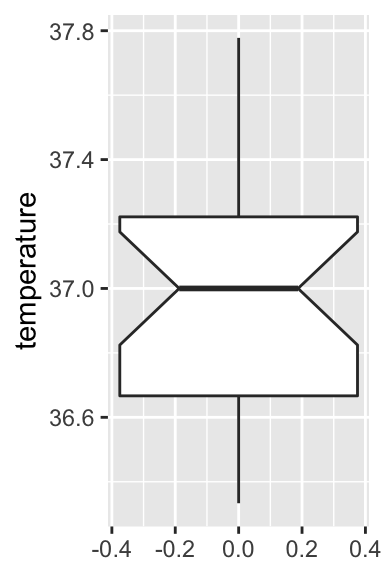
\includegraphics[width=0.25\linewidth]{figure/unnamed-chunk-19-1} \end{center}

Comme pour le stripchart présenté plus haut, l'axe des abscisses n'a ici aucun sens. Nous n'avons qu'une unique série de données, l'axe des \texttt{x} est donc inutile et nous pouvons donc le retirer :

\begin{Shaded}
\begin{Highlighting}[]
\NormalTok{Temp_clean }\OperatorTok\StringTok{ }
\StringTok{  }\KeywordTok{ggplot}\NormalTok{(}\KeywordTok{aes}\NormalTok{(}\DataTypeTok{y =}\NormalTok{ temperature)) }\OperatorTok{+}
\StringTok{  }\KeywordTok{geom_boxplot}\NormalTok{(}\DataTypeTok{notch =} \OtherTok{TRUE}\NormalTok{) }\OperatorTok{+}
\StringTok{  }\KeywordTok{theme}\NormalTok{(}\DataTypeTok{axis.text.x =} \KeywordTok{element_blank}\NormalTok{(),}
        \DataTypeTok{axis.ticks.x =} \KeywordTok{element_blank}\NormalTok{())}
\end{Highlighting}
\end{Shaded}

\begin{center}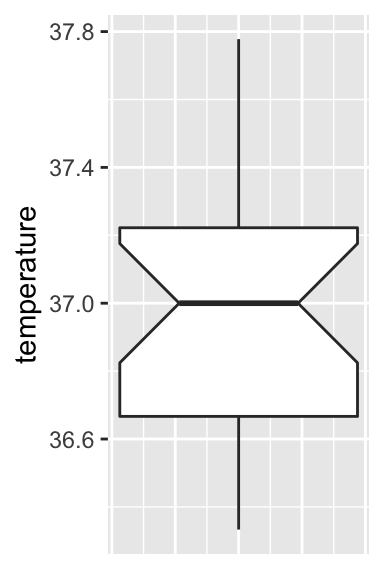
\includegraphics[width=0.25\linewidth]{figure/unnamed-chunk-20-1} \end{center}

On retrouve sur ce graphique tous les éléments obtenus avec la fonction \texttt{summary()} à l'exception de la moyenne. Assurez-vous que vous êtes bien capables d'identifier tous ces éléments sur le graphique. Assurez-vous aussi que la signification de l'encoche (obtenue avec l'argument \texttt{notch\ =\ TRUE}) est bien claire pour vous. Comme toujours, si ce n'est pas le cas, consultez \href{https://besibo.github.io/DA/viz.html\#les-boites-a-moustaches-ou-boxplots}{la section dédiée aux boxplots} dans le livre en ligne de Biométrie 2.

Pour conclure, ces 3 types de représentations graphiques (nuages de points ou stripchart, histogrammes et boxplots) sont complémentaires. Ces trois types de représentations graphiques permettent de visualiser la distribution d'une variable numérique. Les nuages de points permettent de voir toutes les données brutes. Les histogrammes résument les données en quelques valeurs : une valeur d'abondance pour chaque classe de taille. Les boxplots résument encore plus les données avec seulement 7 valeurs qui caractérisent la distribution :

\begin{figure}[htpb]

{\centering 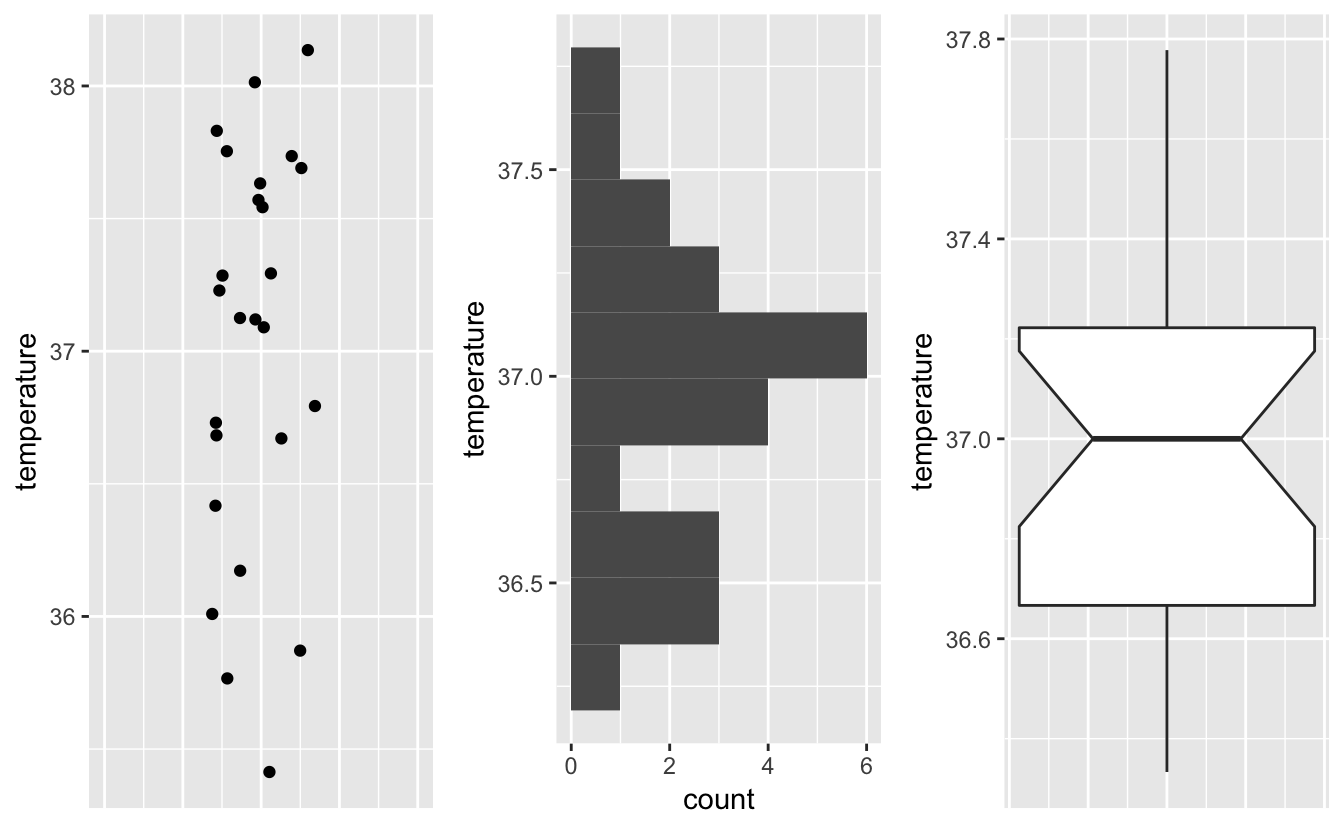
\includegraphics[width=0.9\linewidth]{figure/compboxplot-1} 

}

\caption{Comparaison de 2 types de représentations graphiques}\label{fig:compboxplot}
\end{figure}

À chaque nouvelle analyse statistique, il sera donc important de visualiser les données afin de repérer les éventuels problèmes, et afin d'anticiper sur les résultats que fourniront les tests d'hypothèses ultérieurs. Ici, l'examen de ces graphiques nous permet de dire les choses suivantes :

\begin{enumerate}
\def\labelenumi{\arabic{enumi}.}
\tightlist
\item
  Il n'y a visiblement pas de données aberrantes
\item
  La distribution des données semble suivre à peu près la loi Normale
\item
  La médiane et son intervalle de confiance à 95\% sont centrés sur la valeur 37ºC. Un test devrait donc arriver à la conclusion que la température corporelle des adultes n'est pas significativement différente de 37ºC. Néanmoins, la largeur de l'intervalle de confiance à 95\% est assez grande, ce qui indique une incertitude relativement élevée. Une plus grande quantité de données permettrait certainement d'obtenir plus de précision.
\end{enumerate}

\hypertarget{le-test-parametrique}{%
\subsubsection{Le test paramétrique}\label{le-test-parametrique}}

Le test permettant de comparer la moyenne d'une population à une valeur théorique, fixée par l'utilisateur, est le \textbf{test de Student à un échantillon}. Il s'agit d'un test paramétrique très puissant. Comme tous les tests paramétriques, certaines conditions d'application doivent être vérifiées avant de pouvoir l'appliquer.

\hypertarget{conditions-dapplication}{%
\paragraph{Conditions d'application}\label{conditions-dapplication}}

Les conditions d'application du test de Student à un échantillon sont les suivantes :

\begin{enumerate}
\def\labelenumi{\arabic{enumi}.}
\tightlist
\item
  Les données de l'échantillon sont issues d'un \textbf{échantillonnage aléatoire} au sein de la population générale. Cette condition est partagée par toutes les méthodes que nous verrons dans ces TP. En l'absence d'informations sur la façon dont l'échantillonnage a été réalisé, on considère que cette condition est remplie. Il n'y a pas de moyen statistique de le vérifier, cela fait uniquement référence à la stratégie d'échantillonnage et à la rigueur de la procédure mise en œuvre lors de l'acquisition des données.
\item
  La variable étudiée doit suivre une \textbf{distribution Normale} dans la population générale. Nous allons vérifier cette condition d'application avec un test de Normalité de Shapiro-Wilk.
\end{enumerate}

Comme pour tous les tests statistiques que nous allons réaliser lors de ces séances de TP et TEA, nous devons commencer par spécifier les hypothèses nulles et alternatives aoinsi que la valeur du seuil \(\alpha\) que nous allons utiliser. Ici, nous utiliserons toujours le seuil \(\alpha = 0.05\).

Pour un test de normalité, les hypothèses sont toujours les suivantes :
- H\(_0\) : la variable étudiée suit une distribution Normale dans la population générale.
- H\(_1\) : la variable étudiée ne suit pas une distribution Normale dans la population générale.

Le test de Shapiro-Wilk se réalise de la façon suivante :

\begin{Shaded}
\begin{Highlighting}[]
\NormalTok{Temp_clean }\OperatorTok\StringTok{ }
\StringTok{  }\KeywordTok{pull}\NormalTok{(temperature) }\OperatorTok\StringTok{ }
\StringTok{  }\KeywordTok{shapiro.test}\NormalTok{()}
\end{Highlighting}
\end{Shaded}

\begin{verbatim}

    Shapiro-Wilk normality test

data:  .
W = 0.97216, p-value = 0.7001
\end{verbatim}

\texttt{W} est la statistique du test. Elle permet à RStudio de calculer la \emph{p}-value du test. Ici, \(p > \alpha\). On ne peut donc pas rejeter l'hypothèse nulle de noramlité : on ne peut pas exclure que dans la population générale, la température suive bel et bien une distribution Normale. Les conditions d'application du test de Student sont bien vérifiées.

\hypertarget{realisation-du-test-et-interpretation}{%
\paragraph{Réalisation du test et interprétation}\label{realisation-du-test-et-interpretation}}

Puisque les conditions d'application du test de Student à un échantillon sont vérifiées, nous devons maintenant spécifier les hypothèses nulles et alternatives que nous allons utiliser pour réaliser ce test :

\begin{itemize}
\tightlist
\item
  H\(_0\) : dans la population générale, la température corporelle moyenne des adultes en bonne santé vaut 37ºC (\(\mu = 37\)).
\item
  H\(_1\) : dans la population générale, la température corporelle moyenne des adultes en bonne santé est différente de 37ºC (\(\mu \neq 37\)).
\end{itemize}

On réalise ensuite le test de la façon suivante :

\begin{Shaded}
\begin{Highlighting}[]
\NormalTok{Temp_clean }\OperatorTok\StringTok{ }\KeywordTok{pull}\NormalTok{(temperature) }\OperatorTok\StringTok{ }\KeywordTok{t.test}\NormalTok{(}\DataTypeTok{mu =} \DecValTok{37}\NormalTok{)}
\end{Highlighting}
\end{Shaded}

\begin{verbatim}

    One Sample t-test

data:  .
t = -0.56065, df = 24, p-value = 0.5802
alternative hypothesis: true mean is not equal to 37
95 percent confidence interval:
 36.80235 37.11321
sample estimates:
mean of x 
 36.95778 
\end{verbatim}

Sur la première ligne, R nous confirme que nous avons bien réalisé un test de STudent à un échantillon. La prmière ligne de résutats fournit la valeur du \(t\) calculé (ici, -0.56), le nombre de degrés de libertés (ici, \texttt{df} = 24), et la \(p\)-value (ici, 0.58, soit une valeur supérieure à \(alpha\)). Cette première ligne contient donc tous les résultats du test qu'il conviendrait de rappeler dans un rapport. On devrait ainsi dire :

\begin{quote}
Au seuil \(\alpha\) de 5\%, on ne peut pas rejeter l'hypothèse nulle \(\mu = 37\) (\(t = -0.56\), ddl = 24, \(p = 0.58\)). Les données observées sont donc compatibles avec l'hypothèse selon laquelle la température corporelle moyenne des adultes en bonne santé vaut 37ºC.
\end{quote}

C'est de cette manière que vous devriez rapporter les resultats de ce test dans vos comptes-rendus et rapports à partir de maintenant.

Dans les résultats du test, la ligne suivante (\texttt{alternative\ hypothesis:\ ...}) \textbf{ne donne pas la conclusion du test}. Il s'agit simplement d'un rappel concernant l'hypothèse alternative qui a été utilisée pour réaliser le test. Ici, l'hypothèse alternative utilisée est une hypothèse bilatérale (\(\mu \neq 37\)). Nous verrons plus tard comment spécifier des hypothèse alternatives uni-latérales, même si la plupart du temps, mieux vaut s'abstenir de réaliser de tels tests (à moins bien sûr d'avoir une bonne raison de la faire).

Les résultats fournis ensuite concernent non plus le test statistique à proprement parler, mais l'estimation. Ici, la moyenne de l'échantillon est fournie. Il s'agit de la meilleure estimation possible de la moyenne de la population : \(\bar{x} = \hat{\mu} = 36.96\). Comme pour toutes les estimations, cette valeur est entachée d'oncertitude liée à la fluctuation d'échantillonnage. L'intervalle de confiance à 95\% de cette estimation de moyenne est donc également fourni : \([36.80 ; 37.11]\). Autrement dit, cet intervalle contient les valeurs les plus vraissemblables pour la véritable valeur de moyenne dans la population générale. Cela confirme bien que nous n'avons pas prouvé au sens strict que la moyenne de la population vaut 37ºC. Nous avons en réalité montré que nous ne pouvions pas exclure que la moyenne de la population générale soit de 37ºC. Cette valeur est en effet comprise dans l'intervalle de confiance. On ne peut donc pas l'exclure. Mais beaucoup d'autres valeurs figurent aussi dans cet intervalle. Il est donc tout à fait possible que la moyenne soit en réalité différente de 37ºC. Pour en être sûr, il faudrait probablement un échantillon de plus grande taille afin de limiter l'incertitude.

\hypertarget{lalternative-non-parametrique}{%
\subsubsection{L'alternative non paramétrique}\label{lalternative-non-parametrique}}

Si jamais les conditions d'application du test de Student à un échantillon n'étaient pas remplies, il faudrait alors réaliser son équivalent non paramétrique : le \textbf{test de Wilcoxon des rangs signés}. Ce test est moins puissant que son homologue paramétrique. On ne l'effectue donc que lorsque l'on n'a pas le choix :

\begin{Shaded}
\begin{Highlighting}[]
\NormalTok{Temp_clean }\OperatorTok\StringTok{ }\KeywordTok{pull}\NormalTok{(temperature) }\OperatorTok\StringTok{ }\KeywordTok{wilcox.test}\NormalTok{(}\DataTypeTok{mu =} \DecValTok{37}\NormalTok{, }\DataTypeTok{conf.int =} \OtherTok{TRUE}\NormalTok{)}
\end{Highlighting}
\end{Shaded}

\begin{verbatim}
Warning in wilcox.test.default(., mu = 37, conf.int = TRUE): cannot
compute exact p-value with ties
\end{verbatim}

\begin{verbatim}
Warning in wilcox.test.default(., mu = 37, conf.int = TRUE): cannot
compute exact confidence interval with ties
\end{verbatim}

\begin{verbatim}

    Wilcoxon signed rank test with continuity correction

data:  .
V = 143, p-value = 0.6077
alternative hypothesis: true location is not equal to 37
95 percent confidence interval:
 36.77780 37.11114
sample estimates:
(pseudo)median 
      36.94446 
\end{verbatim}

La syntaxe est identique à celle du test de Student à un échantillon à une exception près : l'ajout de l'argument \texttt{conf.int\ =\ TRUE} qui permet d'afficher la (pseudo)médiane de l'échantillon et son intervalle de confiance à 95\%.

Les hypothèses nulles et alternatives de ce test sont les mêmes que celles du test de Student à un échantillon. En toute rigueur, on teste l'égalité de la médiane à une valeur théorique, et non l'égalité de la moyenne. Mais dans la pratique, la grande majorité des utilisateurs de ce test font l'amalgame entre moyenne et médiane. Ici, la conclusion correcte devrait être :

\begin{quote}
Au seuil \(\alpha\) de 5\%, on ne peut pas rejeter l'hypothèse nulle (test de Wilcoxon des rangs signés, \(V\) = 143, \(p\) = 0.6077). La médiane de la population (\(\widehat{med}\) = 36.94) n'est pas significativement différente de 37ºC (IC 95\% : \([36.78 ; 37.11]\)).
\end{quote}

Si les données ne suivent pas la loi Normale, la médiane est bien la métrique la plus intéressante puisque c'est elle qui nous renseigne sur la tendance centrale des données.

Enfin, les tests de Wilcoxon renvoient souvent des messages d'avretissement. Il ne s'agit que de ça : des avertissements. Tant que la \(p\)-value des tests est éloignée de la valeur seuil \(\alpha\), cela n'a pas d'importance. Quand en revanche la \(p\)-value est très proche de \(\alpha\), il faut être très prudent face aux conclusions du test qui peuvent alors être assez ``fragiles''.

(Notez que pour le test de Student à un échantillon comme pour le test de Wilcoxon des rangs signés, les conclusions sont en accord avec nos observations initiales réalisées à partir du boxplot).

\hypertarget{exercice-dapplication}{%
\subsubsection{Exercice d'application}\label{exercice-dapplication}}

Le fichier \texttt{Temperature2.csv} contient les données brutes d'une seconde étude similaire, réalisée à plus grande échelle. Importez ces données et analysez-les afin de vérifier si la température corporelle moyenne des adultes en bonne santé vaut bien 37ºC. Comme toujours, avant de vous lancer dans la réalisation des tests statistiques, prenez le temps d'examiner vos données comme nous l'avons décrit dans la section \ref{Explo}, afin de savoir où vous aller, de repérer les éventuelles données manquantes ou aberrantes.

\hypertarget{comparaison-de-la-moyenne-de-2-populations-donnees-appariees}{%
\subsection{Comparaison de la moyenne de 2 populations : données appariées}\label{comparaison-de-la-moyenne-de-2-populations-donnees-appariees}}

\hypertarget{le-test-parametrique-1}{%
\subsubsection{Le test paramétrique}\label{le-test-parametrique-1}}

\hypertarget{conditions-dapplication-1}{%
\paragraph{Conditions d'application}\label{conditions-dapplication-1}}

\hypertarget{le-test-non-parametrique}{%
\subsubsection{Le test non paramétrique}\label{le-test-non-parametrique}}

\hypertarget{comparaison-de-la-moyenne-de-2-populations-donnees-independantes}{%
\subsection{Comparaison de la moyenne de 2 populations : données indépendantes}\label{comparaison-de-la-moyenne-de-2-populations-donnees-independantes}}

\hypertarget{le-test-parametrique-2}{%
\subsubsection{Le test paramétrique}\label{le-test-parametrique-2}}

\hypertarget{conditions-dapplication-2}{%
\paragraph{Conditions d'application}\label{conditions-dapplication-2}}

\hypertarget{le-test-non-parametrique-1}{%
\subsubsection{Le test non paramétrique}\label{le-test-non-parametrique-1}}

\hypertarget{tests-bilateraux-et-unilateraux}{%
\subsection{Tests bilatéraux et unilatéraux}\label{tests-bilateraux-et-unilateraux}}

\hypertarget{le-test-parametrique-3}{%
\subsubsection{Le test paramétrique}\label{le-test-parametrique-3}}

\hypertarget{le-test-non-parametrique-2}{%
\subsubsection{Le test non paramétrique}\label{le-test-non-parametrique-2}}

\hypertarget{seance-2-analyse-de-variance}{%
\section{Séance 2 : analyse de variance}\label{seance-2-analyse-de-variance}}

\hypertarget{seance-3-correlations-et-regressions}{%
\section{Séance 3 : corrélations et régressions}\label{seance-3-correlations-et-regressions}}

\hypertarget{seance-4-applications-et-corrections}{%
\section{Séance 4 : applications et corrections}\label{seance-4-applications-et-corrections}}

\bibliography{book.bib,packages.bib}


\end{document}
